% !TeX spellcheck = en_US
% !TEX root = ../thesis-example.tex
%
\section{Chroma Key}
\label{sec:chromakey}

Beginning from the camera, the video signal travels through the Inogeni 
converter and is accessible with the systems API for webcams. 
(See figure \ref{fig:system-components})

\begin{figure}[htb]
	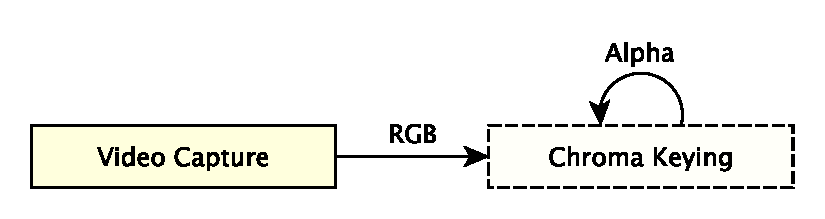
\includegraphics[width=\textwidth]{_raw_resources/pipeline_steps/4_1_chroma.pdf}
	\caption{Initial step upon receiving the camera image}
	\label{fig:steps:chroma}
\end{figure}

The initial step is to remove the green (or blue) background from the image, 
which should be either a green (or blue) box, in this case it is a greenscreen. 
Other literature usually refers to it as "pulling a video matte" or "chroma 
keying". For a reference green, there has to be a color picked manually in the 
material editor of Unity - this was made easy by a checkbox to show raw output 
from the camera. Then a middle-ground green can be picked. This is an important 
setup step, since lightning situations can vary greatly and minor differences 
in light setups can have a great effect on the outcome of visible green 
background captured by the camera.
\newline
An extreme example case is used for comparing these chroma keying variants, 
which shows high motion blue due to a low shutter speed and fast movement of 
the depicted actor:

\begin{figure}[htb]
	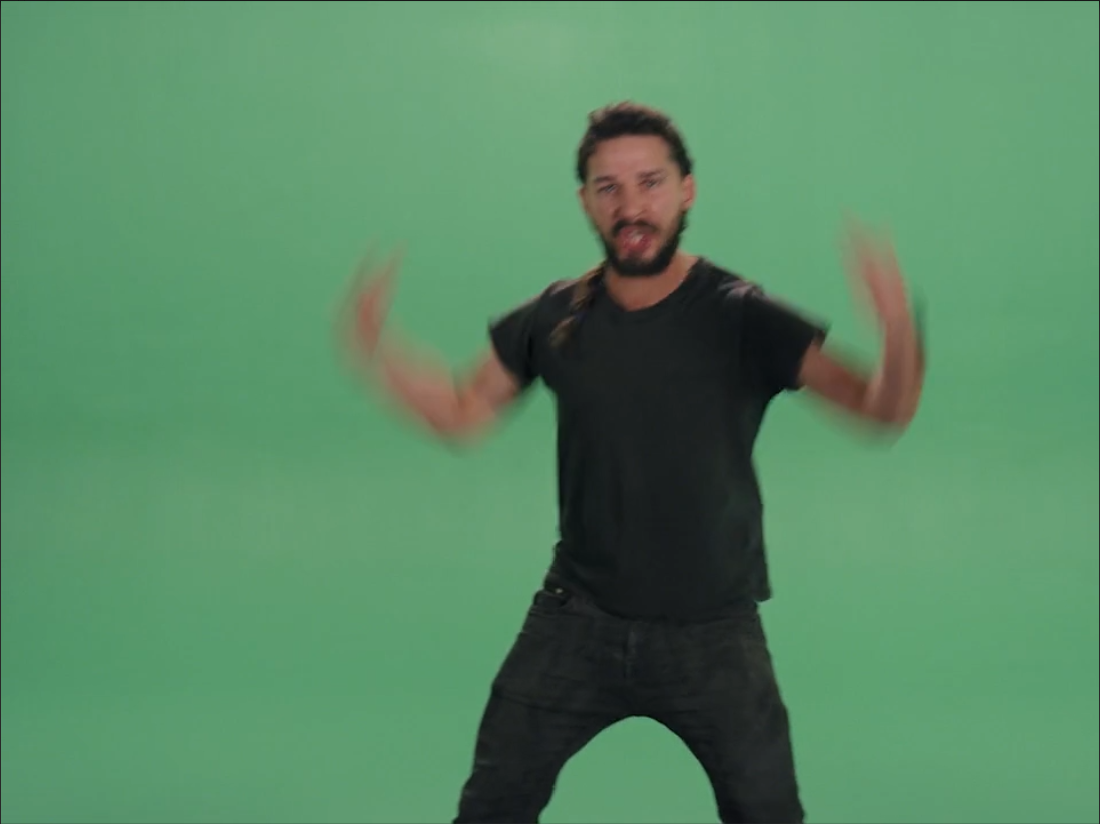
\includegraphics[width=\textwidth]{_raw_resources/Comparison_Example.png}
	\caption{Comparison Image \cite{vimeo:shia:2015} - sRGB Output}
	\label{fig:chroma:color}
\end{figure}

\subsection{Initial Assumption}

Each RGB color can be represented as a discrete 3-Vector of (red, green, blue) 
values in range of $[0, 1]$\footnote{Software RGBA color representations 
usually take 8bit per color channel and map between $[0, 255]$ - graphic 
computing usually maps between $[0, 1]$}. An interpolation between two colors 
can be summarized as matting equation as following, where a foreground image 
$C_F$ and a background image $C_B$ - $\alpha_B$ is assumed to be $1$:

\eq{eq:chroma:assumption:alpha:1}{
	I(x, y) = \alpha(x,y) C_F(x, y) + (1 - \alpha(x, y)) C_B(x, y)
}

This matting equation has to be generalized for a later step, where 
$\protect\alpha$ is a value between [0, 1] on fore- and background, yielding a 
total Alpha of $\alpha_T$ as following:

\eq{eq:chroma:assumption:alpha:weak}{
	\alpha_T = \alpha_B * (1 - \alpha_F) \\
}

thus:

\eq{eq:chroma:assumption:alpha:cont}{
	I(x, y) = (1 - \alpha_T)F(x, y) + \alpha_T B(x, y)
}

\subsection{Euclidean RGB Difference}
Assuming a source pixel color $C_S$ and a reference color $C_R$ we can 
calculate the euclidean distance between these colors.
\eq{eq:euclidianrgb}{
	\alpha = \sqrt{(C_RR - C_SR)^2 + (C_RG - C_SG)^2 + (C_RB - C_SB)^2}
}

This is computationally very low cost and works well enough for tell a 
difference between two separate colors. It fails to accommodate for colors that 
are perceived as different, but are tinted by the reference colors. Since the 
greenscreen material will never achieve 0\% reflectivity, some color will spill 
onto the filmed actor and will therefore generate unwanted chroma-keying 
artifacts, most noticeable on semi-glossy reflection of skin or color tints on 
white clothing.

\begin{figure}[htb]
	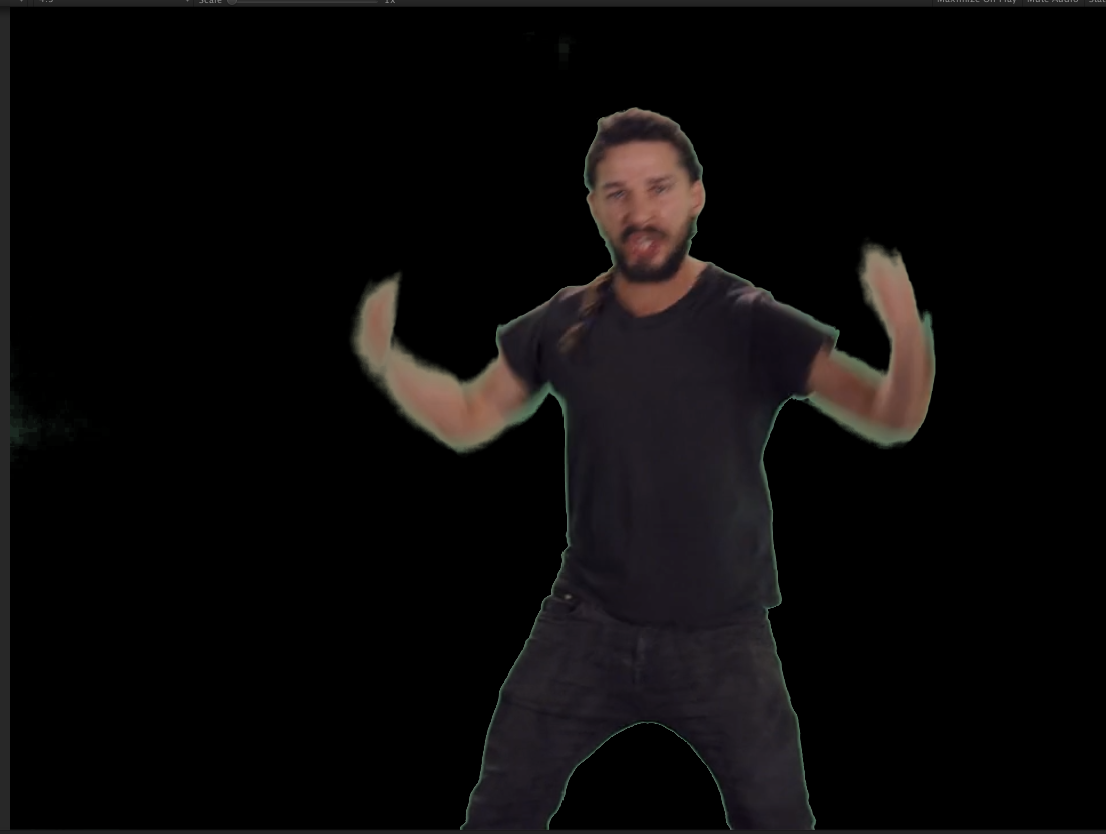
\includegraphics[width=\textwidth]{_raw_resources/Comparison_RGB_color.png}
	\caption{Chroma Keying by using euclidean RGB distance}
	\label{fig:chroma:euclidean:rgb}
\end{figure}

\subsection{Euclidean YCgCo Difference}

YCgCo gets its name for Luminance (Y), chrominance green (Cg) and chrominance 
orange (Co) and helps decorrelating color spaces by splitting color-lightness 
from color chrominances. Since it is a fast, lossless color transformation it 
is used in example for H.264 video encoding and other image compression 
techniques. The two chrominance channels are then split into green to magenta 
and orange to blue color channels and allow for a more accurate distance 
calculation between two colors.
\newline
Transforming any RGB color to YCgCo can done with a single matrix  
multiplication, which is - again - a very low-cost computation on a GPU:

\eq{eq:ycgco:transformation}{
	\begin{bmatrix}
		Y \\
		Cg \\
		Co \\
	\end{bmatrix}
	=
	\begin{bmatrix}
		 \frac{1}{4} && \frac{1}{2} &&  \frac{1}{4} \\
		-\frac{1}{4} && \frac{1}{2} && -\frac{1}{4} \\
		 \frac{1}{2} && 0           && -\frac{1}{2}
	\end{bmatrix}
	*
	\begin{bmatrix}
		R \\
		G \\
		B 
	\end{bmatrix}
}

Given two colors, one from the video source $C_S$ and a reference color $C_R$ 
it is now possible to calculate the euclidean distance on the two chrominance 
channels:

\eq{eq:ycgco:euclidean}{
	\alpha = \sqrt{(C_RCg - C_SCg)^2 + (C_RCo - C_SCo)^2}
}

Since the increased decorrelation, the result is more accurate and shows less 
artifacting on target pixels, allowing for a more accurate matte pulling, less 
green edges and a more continuous image of an actor.

\begin{figure}[htb]
	\includegraphics[width=\textwidth]{_raw_resources/Comparison_YCgCo_color.png}
	\caption{Chroma Keying by using euclidean YCgCo distance}
	\label{fig:chroma:euclidean:ycgco}
\end{figure}

\subsection{Euclidean Lab Difference}
The International Color Consortium (ICC) defined 1976 \textit{Lab $\Delta$E} as 
a standard model of calculating color differences with \textit{Lab} colors. The 
final distance calculation is, too, a linear euclidean distance as with all 
other models, but accommodates for perceived color differences. It is a more 
expensive computation wise and needs in implementation code branches, which 
will both be evaluated by the GPU before using either branching code path.

Since any given RGB color has to be converted to  the Lab color model a 
reference white has to be used to accommodate for different color models. 
Luckily the given webcam signal defaults to sRGB D65 and does not need a 
configurable reference matrix based on a given color model.

\todo[inline]{this is very rough and only contains equations currently used}

sRGB conversion to linear RGB in respect of energy per channel:

\eq{chroma:inversecompanding}{
	v \in \{r, g, b\} \land V \in \{R, G, B\}
}

where: 

\eq{chroma:inverseRGBcompanding}{
	v = \\
	\begin{cases}
		V / 12.92                   & \quad \text{if } V \leq 0.0405 \\
		((V + 0.055) / 1.055)^{2.4} & \quad \text{otherwise}
	\end{cases}
}

from there and RGB to XYZ conversion can be done by:

\eq{chroma:conversioncalc}{
	\begin{bmatrix}
		X\\
		Y\\
		Z\\
	\end{bmatrix}
		=
	\begin{bmatrix}
		M
	\end{bmatrix}
	\begin{bmatrix}
		R\\
		G\\
		B\\
	\end{bmatrix}
}

where:

\eq{chroma:rgbmatrix}{
	\begin{bmatrix}
		M
	\end{bmatrix}
		=
	\begin{bmatrix}
		R X_r && G X_g && B X_b \\
		R Y_r && G Y_g && B Y_b \\
		R Z_r && G Z_g && B Z_b
	\end{bmatrix}
}


\eq{chroma:xyzmatrix}{
		\begin{bmatrix}
		X\\
		Y\\
		Z\\
	\end{bmatrix}
	\begin{bmatrix}
		M
	\end{bmatrix}
	=
	\begin{pmatrix}
		X_r / Y_r && X_g / Y_g && X_b / Y_g \\
		1 && 1 && 1 \\
		\frac{1-X_r-Y_r}{Y_r} && \frac{1-X_g-Y_g}{Y_g} && \frac{1-X_b-Y_b}{Y_b}
	\end{pmatrix}
}

Where $\begin{bmatrix}M\end{bmatrix}$ for RGB D65 is:

\eq{chroma:sRGBD65}{
	\begin{bmatrix}
		0.4124564 && 0.3575761 && 0.1804375 \\
		0.2126729 && 0.7151522 && 0.0721750 \\
		0.0193339 && 0.1191920 && 0.9503041 \\
	\end{bmatrix}
}

Based on a reference white $U_r \in \{X_r, Y_r, Z_r\}$:

\eq{chroma:xyz2lab:defines}{
	U \in \{X, Y, Z\} \land W \in \{L, a, b\}
}

\eq{chroma:xyz2lab:epsilon}{
	\epsilon = 0.008856 \land \kappa = 903.3
}

where:

\eq{chroma:xyz2lab:ref}{
	w_r = \frac{U}{U_r}
}

\eq{chroma:xyz2lab:channel}{
	f(w) = \\
	\begin{cases}
		\sqrt[3]{w_r}      & \quad \text{if } U > \epsilon \\
		\frac{\kappa w_r + 16}{116} & \quad \text{otherwise}
	\end{cases}
}


\eq{chroma:xyz2lab:conversion}{
	\begin{bmatrix}
		L \\
		a \\
		b \\
	\end{bmatrix}
	=
	\begin{bmatrix}
		116 f_y - 16 \\
		500 (f_x - f_y) \\
		200 (f_y - f_z)
	\end{bmatrix}
}

With this conversion from sRGB to linear RGB to XYZ to Lab we can now calculate 
the euclidian linear distance between two colors $C_1$ and $C_2$, which already 
have been converted to Lab:

\eq{chroma:cie76:distance}{
	\Delta E = \sqrt{(C_2L - C_1L)^2 + (C_2a - C_1a)^2 + (C_2b - C_1b)^2}
}

These values are rated by their perceptive difference \cite{mokrzycki:2012}:

\begin{tabular}{l | l}
	0.0 \dots 0.5 & the difference is unnoticeable \\
	0.5 \dots 1.0 & the difference is only noticed by an experienced observer \\
	1.0 \dots 2.0 & the difference is also noticed by an unexperienced observer 
	\\
	2.0 \dots 4.0 & the difference is clearly noticeable \\
	4.0 \dots 5.0 & fundamental color difference  \\
	> 5.0 		  & gives the impression that these are two different 
	colors        
\end{tabular}

Now it's possible to map alpha values for each pixel based on $\Delta$E 
distances between $m, n$ by clamping and biasing $\Delta$E:

\eq{chroma:cie76:clamp}{
	f({\Delta E}) = x = \frac{\Delta E - n}{m - n}
}

\eq{chroma:cie76:min/max}{
	\alpha_{\Delta E} =
	\begin{cases}
		n        & \quad \text{if } x \leq n \\
		x        & \quad \text{if } n \leq x \leq m \\
		m        & \quad \text{if } m \leq x
	\end{cases}
}

\eq{chroma:cie76:mapping}{
	\alpha(I(x, y)) = 3\Delta E^2 - 2\Delta E^3
}

With that we receive a more natural matte with nearly no green edges, 
continuous actor imagery. Motion blur is hard to account for and is even with 
professional video matting hardware, extensive post production or intrinsic 
frame matting hard to remove without very rough image results.

\begin{figure}[htb]
	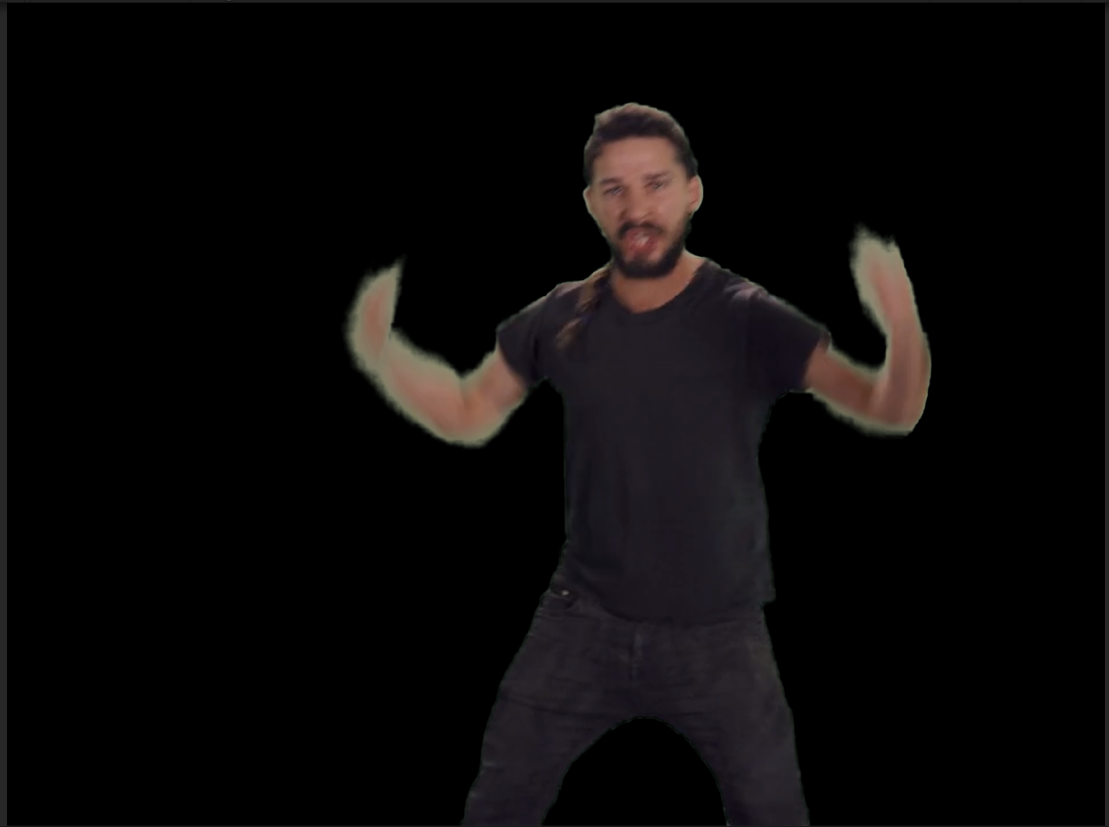
\includegraphics[width=\textwidth]{_raw_resources/Comparison_DeltaE_color.png}
	\caption{Chroma Keying by using $\protect\Delta $E distance}
	\label{fig:chroma:deltae}
\end{figure}

